\chapter{Bloedglucose en diabetes}\label{ch:g12:glucose-and-diabetes}

Vijf liter bloed, één gram glucose in elke liter: vijf gram in totaal,
ongeveer een suikerklontje. Alleen de hersenen al verbranden die
hoeveelheid elk uur, dag en nacht, en kunnen niets anders gebruiken. Toch
houdt iemand die een dag lang niets eet, of in één keer een hele taart
opeet, de concentratie op enkele tienden van een gram per liter na op
dezelfde waarde --- en iemand van wie de alvleesklier het heeft laten
afweten niet, met gevolgen die van dorst tot coma reiken. Dit hoofdstuk
gaat over het nauwkeurigst bewaakte getal van het lichaam, de organen die
het vasthouden, en wat er in de twee vormen van \omterm{def:g12:glucose-and-diabetes:diabetes}{diabetes} gebeurt wanneer
zij dat niet kunnen.

\section{Een geregelde constante}

\begin{definition}[Bloedglucosespiegel]\label{def:g12:glucose-and-diabetes:glycaemia}
De \emph{bloedglucosespiegel}\index{bloedglucosespiegel} is de
concentratie glucose in het bloedplasma: ongeveer \qty{1}{g/L}
(\qty{5.5}{mmol/L}) vóór een maaltijd bij een gezond mens, oplopend tot
\qty{1.4}{g/L} binnen een uur na het eten en binnen twee uur weer terug,
en dalend tot \qty{0.7}{g/L} na een dag vasten. Onder \qty{0.5}{g/L}
falen de hersenen (verwarring, dan coma); boven \qty{1.8}{g/L} lekt er
glucose in de urine, en jaren boven \qty{1.3}{g/L} beschadigen vaten en
zenuwen. De bloedglucosespiegel is een \emph{geregelde} grootheid: een
waarde die bij een streefwaarde wordt gehouden door een stelsel dat haar
meet en bijstuurt.
\end{definition}

\begin{proposition}[De glucosevoorraad en haar stromen]\label{prop:g12:glucose-and-diabetes:pool}
De \qty{5}{g} glucose in het bloed vormen een voorraad waar grote stromen
doorheen gaan. \emph{Toevoer}: de darm na een maaltijd (tot \qty{100}{g}
in een uur), en tussen de maaltijden de \emph{lever}, die glucose afgeeft
uit haar opgeslagen \emph{\omterm{def:g10:exercise-and-energy:glycogen}{glycogeen}} (\qty{100}{g}, een halve dag
voorraad) en nieuwe glucose maakt uit \omterm{def:g10:chemistry-of-life:families}{aminozuren} en lactaat.
\emph{Afvoer}: de hersenen (\qty{5}{g/h}, constant), de spieren (van
enkele grammen tot \qty{100}{g/h} bij inspanning), andere weefsels, en de
opslag als \omterm{def:g10:exercise-and-energy:glycogen}{glycogeen} in de lever en de spieren of als vet. Een voorraad
van \qty{5}{g} die met tientallen grammen per uur wordt gevuld en
geleegd, is alleen stabiel omdat de stromen van minuut tot minuut worden
bijgesteld.
\end{proposition}
\admitted

\begin{omfigure}
\begin{tikzpicture}[font=\small, >=Stealth,
  b/.style={draw, rounded corners, align=center, minimum height=1.0cm}]
  \node[b, fill=omThm!15, text width=3.0cm, minimum height=1.6cm] (blood) at (0,0) {bloedglucose\\ \qty{5}{g}, ongeveer \qty{1}{g/L}};
  \node[b, fill=omDef!12, text width=2.6cm] (gut) at (-4.5,1.6) {darm\\ (na maaltijden)};
  \node[b, fill=omDef!12, text width=2.6cm] (liver) at (-4.5,-1.6) {lever: voorraad\\ glycogeen, nieuwe glucose};
  \node[b, fill=omMeth!15, text width=2.6cm] (brain) at (4.5,1.6) {hersenen: \qty{5}{g/h},\\ alleen glucose};
  \node[b, fill=omMeth!15, text width=2.6cm] (muscle) at (4.5,0) {spieren: gebruik, en\\ opslag als glycogeen};
  \node[b, fill=omMeth!15, text width=2.6cm] (fat) at (4.5,-1.6) {vetweefsel:\\ opslag als vet};
  \draw[->, thick] (gut) -- (blood.west |- 0,0.5);
  \draw[<->, thick] (liver) -- node[below=1pt, font=\scriptsize, sloped] {beide kanten op} (blood.west |- 0,-0.5);
  \draw[->, thick] (blood.east |- 0,0.5) -- (brain);
  \draw[->, thick] (blood.east) -- (muscle);
  \draw[->, thick] (blood.east |- 0,-0.5) -- (fat);
\end{tikzpicture}

{\small De glucosevoorraad. Maaltijden en de lever vullen haar; de
hersenen, de spieren en het vetweefsel legen haar; alleen de lever kan
beide kanten op werken, door na een maaltijd op te slaan en tussen de
maaltijden af te geven.}
\end{omfigure}

\begin{example}[Een dag bloedglucose]\label{ex:g12:glucose-and-diabetes:day}
Ontbijt om 8 uur: de spiegel stijgt van \num{0.9} tot \qty{1.3}{g/L} tegen
9 uur en is om 10 uur terug op \num{1.0}, waarbij het overschot in het
\omterm{def:g10:exercise-and-energy:glycogen}{glycogeen} van lever en spieren is verdwenen. Van 10 tot 13 uur geeft de
lever \omterm{def:g10:exercise-and-energy:glycogen}{glycogeen} af en blijft de waarde rond \num{0.9}. Een rondje hardlopen
om 17 uur trekt in een uur \qty{60}{g} de spieren in; de lever leegt de
helft van haar voorraad om bij te blijven, en de waarde zakt naar
\num{0.8}. 's Nachts maakt de lever nieuwe glucose uit \omterm{def:g10:chemistry-of-life:families}{aminozuren}, en om 7
uur is de waarde \qty{0.9}{g/L}. Er is driehonderd gram door een voorraad
van vijf gegaan.
\end{example}

\section{De alvleesklier houdt de balans}

\begin{proposition}[Twee hormonen uit de eilandjes]\label{prop:g12:glucose-and-diabetes:hormones}
Verspreid door de alvleesklier, tussen de \omterm{def:g10:cells-common-unit:cell}{cellen} die verteringsenzymen
maken, liggen een miljoen kleine trosjes \omterm{def:g10:cells-common-unit:cell}{cellen}, de \emph{eilandjes}\index{eilandjes van de alvleesklier}.
Hun \omterm{def:g10:cells-common-unit:cell}{cellen} meten de \omterm{def:g12:glucose-and-diabetes:glycaemia}{bloedglucosespiegel} van het bloed dat langsstroomt en
scheiden er twee \omterm{def:g11:hormones-and-reproduction:hormone}{hormonen} in af:
\begin{itemize}
  \item \emph{insuline}\index{insuline}, uit de $\beta$-cellen, wanneer de
        spiegel stijgt: zij laat spier- en vetcellen glucose opnemen, en
        de lever en de spieren haar als \omterm{def:g10:exercise-and-energy:glycogen}{glycogeen} opslaan; de spiegel
        daalt;
  \item \emph{glucagon}\index{glucagon}, uit de $\alpha$-cellen, wanneer
        zij daalt: het laat de lever \omterm{def:g10:exercise-and-energy:glycogen}{glycogeen} afbreken en glucose
        afgeven; de spiegel stijgt.
\end{itemize}
De twee werken op dezelfde organen in tegengestelde richting; hun
verhouding, om de paar minuten opnieuw ingesteld door de gemeten spiegel,
is de regeling. \omterm{prop:g12:glucose-and-diabetes:hormones}{Insuline} is het enige \omterm{def:g11:hormones-and-reproduction:hormone}{hormoon} dat de \omterm{def:g12:glucose-and-diabetes:glycaemia}{bloedglucosespiegel}
verlaagt; verscheidene verhogen haar.
\end{proposition}
\begin{proof}[Bewijsmateriaal]
De alvleesklier van een hond weghalen (1889) maakt hem binnen een dag
suikerziek: zijn spiegel verdrievoudigt en er verschijnt glucose in zijn
urine; de buis afbinden die de verteringsenzymen afvoert doet dat niet,
dus is het gevolg niet van de vertering. Een uittreksel van de \omterm{prop:g12:glucose-and-diabetes:hormones}{eilandjes}
inspuiten (1921) verlaagt binnen enkele uren de spiegel van een
suikerzieke hond, en van een suikerziek kind; de werkzame stof, de
\omterm{prop:g12:glucose-and-diabetes:hormones}{insuline}, werd hetzelfde jaar gezuiverd. Losgemaakte \omterm{prop:g12:glucose-and-diabetes:hormones}{eilandjes} in een
schaaltje scheiden \omterm{prop:g12:glucose-and-diabetes:hormones}{insuline} af wanneer de glucose van het medium wordt
verhoogd en \omterm{prop:g12:glucose-and-diabetes:hormones}{glucagon} wanneer zij wordt verlaagd. Ingespoten \omterm{prop:g12:glucose-and-diabetes:hormones}{glucagon}
verhoogt binnen enkele minuten de spiegel van iemand die vast, en alleen
als de lever \omterm{def:g10:exercise-and-energy:glycogen}{glycogeen} bezit.
\end{proof}

\begin{omfigure}
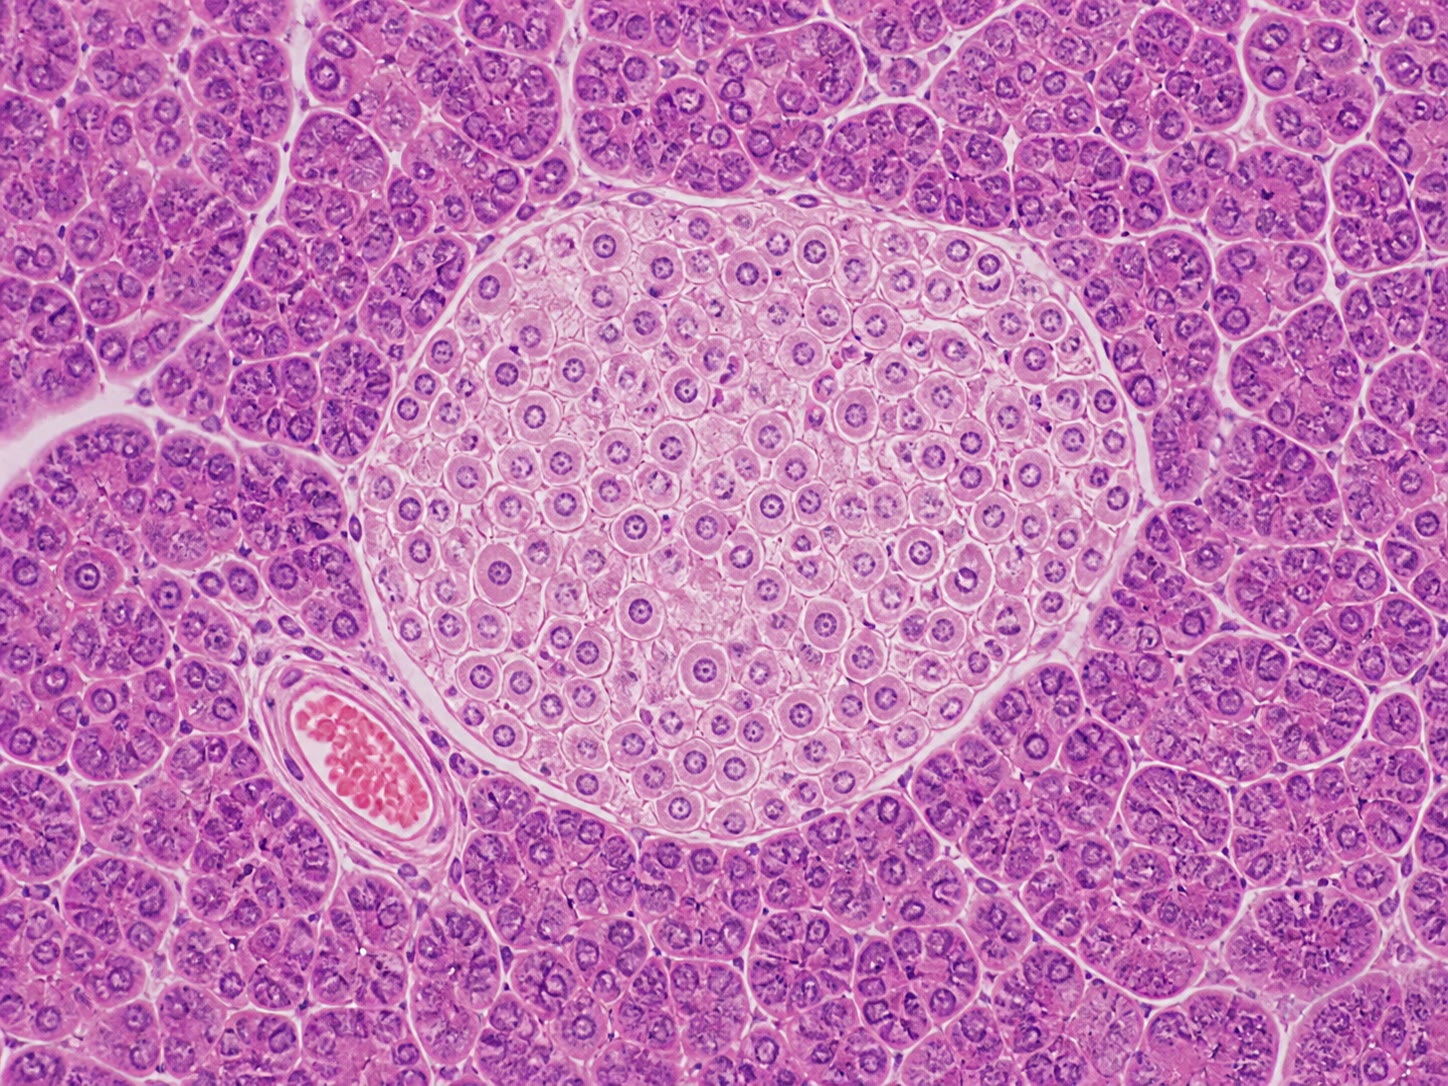
\includegraphics[width=0.56\linewidth]{images/book2/ai/g12-glucose-pancreas-islet.jpg}

{\small Een doorsnede van de alvleesklier: een \omterm{prop:g12:glucose-and-diabetes:hormones}{eilandje}, bleker, tussen de
donkerder trosjes \omterm{def:g10:cells-common-unit:cell}{cellen} die \omterm{def:g11:enzymes-and-phenotype:enzyme}{enzymen} afscheiden. De \omterm{def:g10:cells-common-unit:cell}{cellen} van het
\omterm{prop:g12:glucose-and-diabetes:hormones}{eilandje} lezen de glucose van het bloed af en antwoorden met \omterm{prop:g12:glucose-and-diabetes:hormones}{insuline} of
\omterm{prop:g12:glucose-and-diabetes:hormones}{glucagon}; de rest van het orgaan maakt verteringssap.}
\end{omfigure}

\begin{omfigure}
\begin{tikzpicture}[font=\small, >=Stealth,
  b/.style={draw, rounded corners, align=center, minimum height=1.0cm}]
  \node[b, fill=omThm!15, text width=3.2cm, minimum height=1.4cm] (gly) at (0,0) {bloedglucose\\ (streefwaarde \qty{1}{g/L})};
  \node[b, fill=omProp!15, text width=2.8cm] (beta) at (-4.6,2.0) {$\beta$-cellen: insuline};
  \node[b, fill=omProp!15, text width=2.8cm] (alpha) at (-4.6,-2.0) {$\alpha$-cellen: glucagon};
  \node[b, fill=omMeth!15, text width=3.4cm] (store) at (5.6,2.2) {lever, spier, vet:\\ nemen glucose op en slaan haar op};
  \node[b, fill=omMeth!15, text width=3.4cm] (rel) at (5.6,-2.2) {lever: breekt glycogeen\\ af, geeft glucose af};
  \draw[->, thick] (gly.west |- 0,0.4) -- node[above, sloped, font=\scriptsize] {stijging gemerkt} (beta.east);
  \draw[->, thick] (gly.west |- 0,-0.4) -- node[below, sloped, font=\scriptsize] {daling gemerkt} (alpha.east);
  \draw[->, thick, omProp] (beta.north) -- ++(0,0.6) -| (store.north);
  \draw[->, thick, omProp] (alpha.south) -- ++(0,-0.6) -| (rel.south);
  \draw[->, thick, omThm] (store.west) -- node[above, sloped, font=\scriptsize, align=center] {spiegel\\ daalt $(-)$} (gly.east |- 0,0.4);
  \draw[->, thick, omThm] (rel.west) -- node[below, sloped, font=\scriptsize, align=center] {spiegel\\ stijgt $(+)$} (gly.east |- 0,-0.4);
  \node[font=\scriptsize, anchor=south] at (0,3.3) {insuline};
  \node[font=\scriptsize, anchor=north] at (0,-3.3) {glucagon};
\end{tikzpicture}

{\small De regeling van de \omterm{def:g12:glucose-and-diabetes:glycaemia}{bloedglucosespiegel}. Een stijging roept
\omterm{prop:g12:glucose-and-diabetes:hormones}{insuline} op, die de weefsels glucose laat opslaan en de waarde omlaag
brengt; een daling roept \omterm{prop:g12:glucose-and-diabetes:hormones}{glucagon} op, dat de lever glucose laat afgeven en
haar omhoog brengt. Het gevolg van elk \omterm{def:g11:hormones-and-reproduction:hormone}{hormoon} neemt het signaal weg dat
het opriep: twee lussen van negatieve \omterm{def:g11:hormones-and-reproduction:hormone}{terugkoppeling} rond één
streefwaarde.}
\end{omfigure}

\begin{example}[De lus aan het werk]\label{ex:g12:glucose-and-diabetes:loop}
Na een maaltijd klimt de spiegel; binnen enkele minuten geven de
$\beta$-cellen \omterm{prop:g12:glucose-and-diabetes:hormones}{insuline} af, openen de spieren en de vetcellen hun
glucosepoorten, schakelt de lever over op \omterm{def:g10:exercise-and-energy:glycogen}{glycogeen} maken, en zakt de
waarde terug --- waarop ook de afgifte van \omterm{prop:g12:glucose-and-diabetes:hormones}{insuline} daalt. Tussen de
maaltijden wordt de neiging omlaag door \omterm{prop:g12:glucose-and-diabetes:hormones}{glucagon} beantwoord, wordt er
\omterm{def:g10:exercise-and-energy:glycogen}{glycogeen} afgebroken, en houdt de waarde stand. Geen van beide \omterm{def:g11:hormones-and-reproduction:hormone}{hormonen}
is ooit afwezig; hun verhouding schuift, en de \omterm{def:g12:glucose-and-diabetes:glycaemia}{bloedglucosespiegel} volgt
haar binnen een smalle band.
\end{example}

\section{Wanneer de lus faalt: diabetes}

\begin{definition}[Diabetes]\label{def:g12:glucose-and-diabetes:diabetes}
\emph{Diabetes}\index{diabetes} is een blijvend teveel aan
\omterm{def:g12:glucose-and-diabetes:glycaemia}{bloedglucose}: boven \qty{1.26}{g/L} nuchter, of boven \qty{2}{g/L} twee
uur na een standaardhoeveelheid glucose. De vroege tekenen volgen uit dat
teveel: glucose in de urine, die water met zich meesleept (veel urine,
dorst), en gewichtsverlies wanneer \omterm{def:g10:cells-common-unit:cell}{cellen} de glucose om hen heen niet
kunnen gebruiken. De late schade --- aan de kleine vaten van oog en nier,
aan zenuwen, aan de slagaders --- komt van jaren waarin glucose met
\omterm{def:g10:chemistry-of-life:families}{eiwitten} reageert. Twee ziekten delen die naam.
\end{definition}

\begin{proposition}[Type 1 en type 2]\label{prop:g12:glucose-and-diabetes:types}
\begin{itemize}
  \item \emph{\omterm{def:g12:glucose-and-diabetes:diabetes}{Diabetes} type 1} (ongeveer 10\% van de gevallen) is de
        vernietiging van de $\beta$-cellen door het eigen afweersysteem
        van de patiënt, meestal op kinder- of jeugdleeftijd: de \omterm{prop:g12:glucose-and-diabetes:hormones}{insuline}
        ontbreekt. De spiegel stijgt ongeremd, er wordt vet verbrand bij
        gebrek aan bruikbare glucose en de zure producten daarvan hopen
        zich op; zonder ingespoten \omterm{prop:g12:glucose-and-diabetes:hormones}{insuline} is de ziekte binnen enkele
        maanden dodelijk. De behandeling is \omterm{prop:g12:glucose-and-diabetes:hormones}{insuline}, meermaals per dag,
        gedoseerd op de maaltijden en de gemeten spiegel, levenslang.
  \item \emph{\omterm{def:g12:glucose-and-diabetes:diabetes}{Diabetes} type 2} (ongeveer 90\%) ontwikkelt zich bij
        volwassenen, meestal met overgewicht en weinig beweging: de
        weefsels reageren steeds minder op \omterm{prop:g12:glucose-and-diabetes:hormones}{insuline}
        (\emph{insulineresistentie}), de $\beta$-cellen maken dat goed
        door er meer af te scheiden, en na jaren raken zij uitgeput. De
        \omterm{prop:g12:glucose-and-diabetes:hormones}{insuline} is er wel maar volstaat niet. De aanleg is deels
        erfelijk (\cref{ch:g11:genes-and-disease}); de aanleiding is de
        manier van leven, en de eerste behandeling is die veranderen ---
        afvallen en bewegen --- vóór medicijnen en, laat, \omterm{prop:g12:glucose-and-diabetes:hormones}{insuline}.
\end{itemize}
\end{proposition}
\begin{proof}[Bewijsmateriaal]
Patiënten met type 1 hebben jaren vóór de klachten al antistoffen tegen
hun eigen eilandjescellen, en bij de diagnose zijn hun \omterm{prop:g12:glucose-and-diabetes:hormones}{eilandjes} vrijwel
leeg van $\beta$-cellen en doortrokken van witte bloedcellen; hun \omterm{prop:g12:glucose-and-diabetes:hormones}{insuline}
in het bloed is niet te meten en zij reageren meteen op ingespoten
\omterm{prop:g12:glucose-and-diabetes:hormones}{insuline}. Patiënten met type 2 hebben bij de diagnose een normale of hoge
\omterm{prop:g12:glucose-and-diabetes:hormones}{insuline}; hun spier- en vetcellen nemen bij eenzelfde hoeveelheid \omterm{prop:g12:glucose-and-diabetes:hormones}{insuline}
minder glucose op dan die van een gezond mens; eeneiige tweelingen delen
de ziekte in 70\% van de gevallen, en afvallen of alleen al een
wandelprogramma herstelt bij vele vroege gevallen een normale spiegel.
\end{proof}

\begin{omfigure}
\begin{tikzpicture}
\begin{axis}[
  width=0.88\linewidth, height=5.8cm,
  axis x line=bottom, axis y line=left,
  xmin=0, xmax=180, ymin=0, ymax=3,
  xlabel={minuten na het drinken van \qty{75}{g} glucose}, ylabel={bloedglucose (g/L)},
  xlabel style={font=\small, at={(axis description cs:0.5,-0.12)}, anchor=north},
  ylabel style={font=\small},
  tick label style={font=\small}, xtick={0,30,60,90,120,150,180}, ytick={0,1,2,3},
  legend style={at={(0.5,-0.3)}, anchor=north, legend columns=3, font=\small, draw=none},
  clip=false,
]
\addplot[thick, omMeth, smooth] coordinates {(0,0.9) (30,1.4) (60,1.3) (90,1.1) (120,0.95) (150,0.9) (180,0.9)};
\addplot[thick, omProp, smooth] coordinates {(0,1.1) (30,1.7) (60,1.9) (90,1.85) (120,1.7) (150,1.5) (180,1.35)};
\addplot[thick, omThm, smooth] coordinates {(0,1.6) (30,2.3) (60,2.7) (90,2.8) (120,2.7) (150,2.6) (180,2.5)};
\draw[dashed, gray] (axis cs:0,2) -- (axis cs:180,2);
\node[font=\scriptsize, gray, anchor=south east] at (axis cs:180,2.02) {drempel op 120 min};
\legend{gezond, verminderde tolerantie, diabetes type 2}
\end{axis}
\end{tikzpicture}

{\small De glucosetolerantietest: de \omterm{def:g12:glucose-and-diabetes:glycaemia}{bloedglucosespiegel} na een
standaarddrank van \qty{75}{g} glucose. Een gezond mens is binnen twee uur
terug bij \qty{1}{g/L}; een suikerzieke begint hoog, klimt boven
\qty{2}{g/L} en blijft daar. De tussenliggende kromme is het waarschuwende
stadium, dat meestal nog om te keren is.}
\end{omfigure}

\begin{example}[Een dag met type 1 sturen]\label{ex:g12:glucose-and-diabetes:type1}
Een meisje met type 1 meet vóór elke maaltijd haar \omterm{def:g12:glucose-and-diabetes:glycaemia}{bloedglucose} met een
druppel bloed, telt de \omterm{def:g10:chemistry-of-life:families}{koolhydraten} op haar bord, en spuit een dosis snelle
\omterm{prop:g12:glucose-and-diabetes:hormones}{insuline} in die daarmee evenredig is --- ongeveer één eenheid per
\qty{10}{g} --- plus één keer per dag een trage \omterm{prop:g12:glucose-and-diabetes:hormones}{insuline} voor de
achtergrond. Te veel \omterm{prop:g12:glucose-and-diabetes:hormones}{insuline}, of een overgeslagen maaltijd, en de waarde
zakt onder \qty{0.6}{g/L}: zweten, beven, verwarring, in enkele minuten
verholpen met suiker. Te weinig, en de waarde blijft boven \qty{2}{g/L}
met dorst en vermoeidheid, en de vaten lopen in stilte de schade op. Zij
doet met de hand wat haar $\beta$-cellen met \omterm{def:g11:hormones-and-reproduction:hormone}{terugkoppeling} deden.
\end{example}

\begin{omfigure}
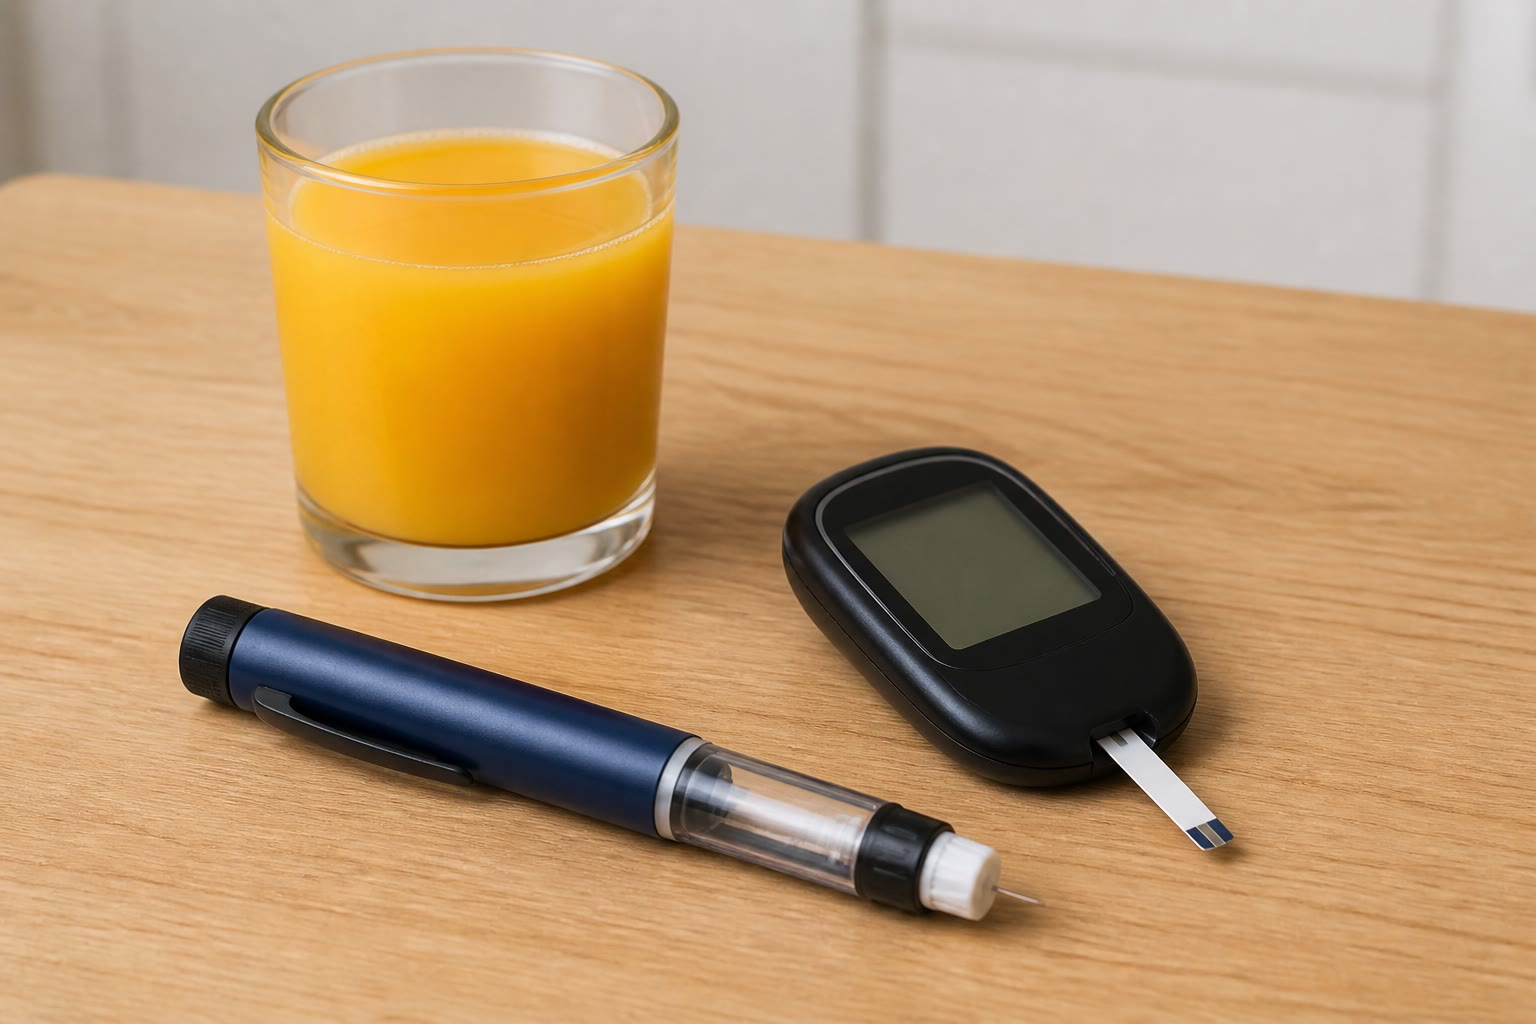
\includegraphics[width=0.56\linewidth]{images/book2/ai/g12-glucose-meter-pen.jpg}

{\small Het gereedschap van iemand met \omterm{def:g12:glucose-and-diabetes:diabetes}{diabetes} type 1: een meter die de
\omterm{def:g12:glucose-and-diabetes:glycaemia}{bloedglucose} uit een druppel bloed afleest, en een pen die een afgemeten
dosis \omterm{prop:g12:glucose-and-diabetes:hormones}{insuline} inspuit. De lus van de \omterm{prop:g12:glucose-and-diabetes:hormones}{eilandjes}, enkele keren per dag met
de hand gedraaid.}
\end{omfigure}

\begin{method}[Een verslag van bloedglucosewaarden lezen]\label{met:g12:glucose-and-diabetes:read}
\begin{enumerate}
  \item Zoek de streefwaarde en de band: nuchter \qtyrange{0.7}{1.1}{g/L},
        na maaltijden onder \num{1.4}; twee uur na een hoeveelheid glucose
        onder \num{1.4} (gezond), \qtyrange{1.4}{2}{} (verminderd), boven
        \qty{2}{g/L} (\omterm{def:g12:glucose-and-diabetes:diabetes}{diabetes}).
  \item Vraag je bij elke stijging af wat er glucose in bracht (maaltijd,
        lever) en wat haar eruit zou moeten halen (de doelwitten van de
        \omterm{prop:g12:glucose-and-diabetes:hormones}{insuline}); bij elke daling, wat haar eruit haalde (hersenen,
        spier) en wat haar terug zou moeten brengen (\omterm{prop:g12:glucose-and-diabetes:hormones}{glucagon}, de lever).
  \item Lees de \omterm{def:g11:hormones-and-reproduction:hormone}{hormonen} samen met de glucose: de \omterm{prop:g12:glucose-and-diabetes:hormones}{insuline} hoort met de
        spiegel te stijgen en het \omterm{prop:g12:glucose-and-diabetes:hormones}{glucagon} te dalen; afwezige \omterm{prop:g12:glucose-and-diabetes:hormones}{insuline}
        betekent type 1, hoge \omterm{prop:g12:glucose-and-diabetes:hormones}{insuline} bij een hoge spiegel betekent
        resistentie.
  \item Reken de eenheden om waar nodig: \qty{1}{g/L} glucose is
        \qty{5.55}{mmol/L}.
\end{enumerate}
\end{method}

\begin{remark}[Een model van regeling]\label{rem:g12:glucose-and-diabetes:model}
Voeler, streefwaarde, twee tegengestelde uitvoerders, negatieve
\omterm{def:g11:hormones-and-reproduction:hormone}{terugkoppeling}: de regeling van de \omterm{def:g12:glucose-and-diabetes:glycaemia}{bloedglucose} heeft hetzelfde ontwerp als
de regeling van het testosteron in
\cref{ch:g11:hormones-and-reproduction}, en als het ontwerp van de meeste
constanten van het lichaam --- temperatuur, water, bloeddruk, zuurgraad.
\omterm{def:g12:glucose-and-diabetes:diabetes}{Diabetes} is hoe een geregelde constante eruitziet wanneer haar lus is
gebroken: de waarde reageert nog altijd op wat er binnenkomt, maar niets
brengt haar terug. De krommen van dit hoofdstuk lezen is oefening in het
lezen van elk van hen.
\end{remark}

\section{Oefeningen}

\begin{exercise}[$\star$]\label{exo:g12:glucose-and-diabetes:1}
Geef de normale nuchtere \omterm{def:g12:glucose-and-diabetes:glycaemia}{bloedglucosespiegel} in \unit{g/L} en in
\unit{mmol/L}, en de twee gevaargrenzen.
\end{exercise}

\begin{exercise}[$\star$]\label{exo:g12:glucose-and-diabetes:2}
Noem de twee \omterm{def:g11:hormones-and-reproduction:hormone}{hormonen} van de \omterm{prop:g12:glucose-and-diabetes:hormones}{eilandjes}, de \omterm{def:g10:cells-common-unit:cell}{cellen} die hen maken, en het
gevolg van elk voor de \omterm{def:g12:glucose-and-diabetes:glycaemia}{bloedglucosespiegel}.
\end{exercise}

\begin{exercise}[$\star$]\label{exo:g12:glucose-and-diabetes:3}
Welk orgaan kan glucose zowel opslaan als afgeven? In welke vorm slaat het
haar op?
\end{exercise}

\begin{exercise}[$\star$]\label{exo:g12:glucose-and-diabetes:4}
Noem in telkens één zin het wezenlijke verschil tussen \omterm{def:g12:glucose-and-diabetes:diabetes}{diabetes} type 1 en
type 2.
\end{exercise}

\begin{exercise}[$\star$]\label{exo:g12:glucose-and-diabetes:5}
Lees in de figuur van de tolerantietest de drie krommen op 120 minuten af
en deel elk in.
\end{exercise}

\begin{exercise}[$\star\star$]\label{exo:g12:glucose-and-diabetes:6}
De hersenen gebruiken \qty{5}{g} glucose per uur en het bloed bevat er
\qty{5}{g}. Leg uit waarom iemand een uur na een maaltijd niet buiten
bewustzijn raakt, en noem het orgaan en het \omterm{def:g11:hormones-and-reproduction:hormone}{hormoon} die daarvoor zorgen.
\end{exercise}

\begin{exercise}[$\star\star$]\label{exo:g12:glucose-and-diabetes:7}
Leg uit waarom de alvleesklier weghalen \omterm{def:g12:glucose-and-diabetes:diabetes}{diabetes} veroorzaakt en haar buis
afbinden niet, en wat dat laat zien over waar de \omterm{prop:g12:glucose-and-diabetes:hormones}{insuline} wordt gemaakt en
hoe zij reist.
\end{exercise}

\begin{exercise}[$\star\star$]\label{exo:g12:glucose-and-diabetes:8}
Iemand die vast krijgt een inspuiting \omterm{prop:g12:glucose-and-diabetes:hormones}{glucagon}: de spiegel stijgt in 20
minuten met \qty{0.4}{g/L}. Dezelfde inspuiting na drie dagen vasten doet
niets. Verklaar dat.
\end{exercise}

\begin{exercise}[$\star\star$]\label{exo:g12:glucose-and-diabetes:9}
Waarom plast iemand met \omterm{def:g12:glucose-and-diabetes:diabetes}{diabetes} veel en heeft hij dorst?
\end{exercise}

\begin{exercise}[$\star\star$]\label{exo:g12:glucose-and-diabetes:10}
Een patiënte met type 1 spuit haar gebruikelijke dosis \omterm{prop:g12:glucose-and-diabetes:hormones}{insuline} in en
slaat dan de lunch over. Voorspel wat er de volgende twee uur gebeurt en
waarom.
\end{exercise}

\begin{exercise}[$\star\star$]\label{exo:g12:glucose-and-diabetes:11}
Leg uit waarom beweging de \omterm{def:g12:glucose-and-diabetes:glycaemia}{bloedglucosespiegel} van iemand met type 2
verlaagt, zelfs zonder enige verandering in de \omterm{prop:g12:glucose-and-diabetes:hormones}{insuline}, met behulp van
\cref{ch:g10:sport-and-health}.
\end{exercise}

\begin{exercise}[$\star\star\star$]\label{exo:g12:glucose-and-diabetes:12}
Twee patiënten hebben nuchter een spiegel van \qty{2}{g/L}. De ene heeft
geen meetbare \omterm{prop:g12:glucose-and-diabetes:hormones}{insuline}; de andere heeft drie keer de normale \omterm{prop:g12:glucose-and-diabetes:hormones}{insuline}.
Stel bij elk de diagnose, en zeg wat de \omterm{prop:g12:glucose-and-diabetes:hormones}{eilandjes} van elke patiënt doen.
\end{exercise}

\begin{exercise}[$\star\star\star$]\label{exo:g12:glucose-and-diabetes:13}
Teken, of beschrijf, de krommen van de \omterm{def:g12:glucose-and-diabetes:glycaemia}{bloedglucose} en van de \omterm{prop:g12:glucose-and-diabetes:hormones}{insuline}
over de drie uur na een maaltijd bij een gezond mens, bij een onbehandelde
patiënt met type 1, en bij een patiënt met type 2. Verklaar elk verschil.
\end{exercise}

\begin{exercise}[$\star\star\star$]\label{exo:g12:glucose-and-diabetes:14}
Een maaltijd bevat \qty{80}{g} \omterm{def:g10:chemistry-of-life:families}{koolhydraten}. Wat zou de
\omterm{def:g12:glucose-and-diabetes:glycaemia}{bloedglucosespiegel} worden als die allemaal in één keer in het bloed
kwamen? Leg uit waarom dat nooit gebeurt, en noem de bestemmingen van de
glucose in de eerste twee uur.
\end{exercise}

\begin{exercise}[$\star\star\star$]\label{exo:g12:glucose-and-diabetes:15}
Vergelijk de regeling van de \omterm{def:g12:glucose-and-diabetes:glycaemia}{bloedglucose} met die van het testosteron in
\cref{ch:g11:hormones-and-reproduction}: voeler, streefwaarde,
uitvoerders, teken van de \omterm{def:g11:hormones-and-reproduction:hormone}{terugkoppeling}. Wat is er bijzonder aan twee
tegengestelde \omterm{def:g11:hormones-and-reproduction:hormone}{hormonen}?
\end{exercise}

\section{Probleem: Vijf gram suiker}

\begin{problem}[{Weekendprobleem --- de glucose van het bloed een dag lang
verantwoord: de voorraad en haar stromen, een tolerantietest gelezen, een
dosis insuline berekend, en een lus die met de hand moet worden
vervangen}]
\label{pb:g12:glucose-and-diabetes:1}
Neem een bloedvolume van \qty{5}{L}, een verbruik van de hersenen van
\qty{5}{g/h} glucose, een voorraad leverglycogeen van \qty{100}{g}, en
spierglycogeen van \qty{400}{g}. Eén eenheid snelle \omterm{prop:g12:glucose-and-diabetes:hormones}{insuline} verwerkt
ongeveer \qty{10}{g} \omterm{def:g10:chemistry-of-life:families}{koolhydraten}.

\medskip
\noindent\textbf{Deel I --- De voorraad.}
\begin{enumerate}
  \item Bereken de massa glucose in het bloed bij \qty{1}{g/L}, en
        dezelfde concentratie in \unit{mmol/L} (glucose
        \qty{180}{g/mol}).
  \item Hoe lang zou de glucose van het bloed alleen de hersenen
        strekken, als er niets voor in de plaats kwam?
  \item Tussen de maaltijden vervangt de lever haar. Hoe lang strekt het
        \omterm{def:g10:exercise-and-energy:glycogen}{glycogeen} van de lever voor de hersenen? Wat gebeurt er daarna?
  \item Het spierglycogeen is vier keer dat van de lever, maar spieren
        kunnen geen glucose aan het bloed afgeven. Leg uit waarom
        spierglycogeen de hersenen niet helpt, en waar het voor dient.
  \item Een maaltijd levert in een uur \qty{60}{g} glucose. Wat zou de
        spiegel bereiken als er niets werd weggehaald? Wat haalt haar
        werkelijk weg, en waar gaat zij heen?
\end{enumerate}

\medskip
\noindent\textbf{Deel II --- De test.}
Een patiënt drinkt \qty{75}{g} glucose. Gemeten \omterm{def:g12:glucose-and-diabetes:glycaemia}{bloedglucose} en \omterm{prop:g12:glucose-and-diabetes:hormones}{insuline}:

\begin{center}
\begin{tabular}{lcccccc}
minuten & 0 & 30 & 60 & 90 & 120 & 180 \\ \hline
\omterm{def:g12:glucose-and-diabetes:glycaemia}{bloedglucose} (g/L) & 1.15 & 1.8 & 2.05 & 2.0 & 1.85 & 1.6 \\
\omterm{prop:g12:glucose-and-diabetes:hormones}{insuline} (\% van een gezonde piek) & 90 & 140 & 180 & 200 & 190 & 160 \\
\end{tabular}
\end{center}
\begin{enumerate}[resume]
  \item Deel de patiënt in met de grenzen van
        \cref{met:g12:glucose-and-diabetes:read}.
  \item Ontbreekt de \omterm{prop:g12:glucose-and-diabetes:hormones}{insuline}? Wat faalt er dan wel?
  \item Noem de ziekte, en geef twee zaken uit de voorgeschiedenis van de
        patiënt die je zou verwachten.
  \item Hoe zou dezelfde tabel eruitzien bij een onbehandelde patiënt met
        type 1?
  \item Welke behandeling wordt als eerste voorgeschreven, en langs welk
        mechanisme werkt zij?
\end{enumerate}

\medskip
\noindent\textbf{Deel III --- De lus met de hand draaien.}
De \omterm{def:g12:glucose-and-diabetes:glycaemia}{bloedglucose} van een patiënte met type 1 is \qty{1.0}{g/L} vóór het
avondeten; de maaltijd bevat \qty{90}{g} \omterm{def:g10:chemistry-of-life:families}{koolhydraten}.
\begin{enumerate}[resume]
  \item Bereken de dosis snelle \omterm{prop:g12:glucose-and-diabetes:hormones}{insuline} voor de maaltijd.
  \item Zij spuit die in maar eet maar de helft van de maaltijd. Schat
        hoe ver de spiegel kan zakken, en noem de klachten en het middel.
  \item Zij spuit niets in en eet de hele maaltijd. Schat de spiegel als
        de \qty{90}{g} allemaal in een voorraad van \qty{5}{L} kwamen, en
        zeg wat de nieren boven \qty{1.8}{g/L} doen.
  \item Waarom moet zij 's nachts, wanneer zij niets eet, ook een trage
        \omterm{prop:g12:glucose-and-diabetes:hormones}{insuline} inspuiten?
  \item Leg uit in welk opzicht de meter en de pen de $\beta$-cel
        vervangen, en wat zij niet kunnen vervangen.
\end{enumerate}

\medskip
\noindent\textbf{Deel IV --- De lus, doordacht.}
\begin{enumerate}[resume]
  \item Een medicijn zet de $\beta$-cellen aan om meer \omterm{prop:g12:glucose-and-diabetes:hormones}{insuline} af te
        scheiden. Bij welk type \omterm{def:g12:glucose-and-diabetes:diabetes}{diabetes} kan het werken, en waarom niet
        bij het andere?
  \item Iemand met type 2 valt \qty{10}{kg} af en wandelt een uur per
        dag; zes maanden later is de tolerantietest normaal. Leg uit welk
        deel van de lus is hersteld.
  \item Leg uit waarom de \omterm{prop:g12:glucose-and-diabetes:hormones}{insuline} en het \omterm{prop:g12:glucose-and-diabetes:hormones}{glucagon} van een gezond mens
        nooit allebei hoog zijn, en wat een \omterm{prop:g12:glucose-and-diabetes:hormones}{eilandje} in een schaaltje doet
        wanneer de glucose van het medium op \qty{1}{g/L} wordt gezet.
  \item \omterm{prop:g12:glucose-and-diabetes:hormones}{Glucagon}, \omterm{prop:g10:heart-lungs-effort:control}{adrenaline}, cortisol en groeihormoon verhogen allemaal
        de \omterm{def:g12:glucose-and-diabetes:glycaemia}{bloedglucose}; alleen \omterm{prop:g12:glucose-and-diabetes:hormones}{insuline} verlaagt haar. Stel voor waarom
        het lichaam verscheidene beveiligingen tegen een lage spiegel
        heeft en één tegen een hoge.
  \item Geef het resultaat: de glucose in het bloed, de uren die de lever
        kan overbruggen, de diagnose van deel II, en de dosis van deel
        III.
\end{enumerate}
\end{problem}
